%-------------------------------------------------------------------------------
%-------------------------------------------------------------------------------
\section{Différentiabilité} \label{sec:Multivar-Diff}
%-------------------------------------------------------------------------------
%-------------------------------------------------------------------------------

% Différentiabilité, définition d’application linéaire tangente.
% Matrice jacobienne, 

On cherche ici à étendre la notion de dérivabilité d'une fonction de $\Rbb$ dans $\Rbb$ à une fonction de $\Rbb^n$ dans $\Rbb^k$. On rappelle d'abord la définition de la dérivabilité pour une fonction de $\Rbb$ dans $\Rbb$.

\begin{definition}[Dérivabilité] \label{def:derivabilite}
  Une fonction $f: \Rbb \mapsto \Rbb$ est dérivable au point $x$ si la limite
  $$
  \lim_{h \rightarrow 0, h \neq 0} \frac{f(x+h) - f(x)}{h}
  $$
  existe. Cette limite est alors la dérivée de $f$ au point $x$. Elle est notée $f'(x)$ et représente la pente de la tangente au graphe de la fonction $f$ au point $x$.
\end{definition}

\remarks
\begin{enumerate}
  \item La limite est définie pour $h \rightarrow 0$, sans spécifier par valeur inférieure ($h \uparrow 0$) ou supérieure ($h \downarrow 0$), ce qui impose que les limites à gauche ($h \uparrow 0$) et à droite ($h \downarrow 0$) soient égales. En dimension supérieure à 1, il sera nécessaire de garantir l'existence d'une même limite dans toutes les directions de l'espace $\Rbb^n$.
  \dessin{Fonction non dérivable, mais dérivable à gauche et à droite}
  \item Cette définition est équivalente à
  $$
  \lim_{h\rightarrow 0, h \neq 0} \frac{f(x+h) - f(x) - hf'(x)}{h} = 0
  \quad \Leftrightarrow \quad 
  \lim_{h\rightarrow 0, h \neq 0} \frac{f(x+h) - f(x) - hf'(x)}{|h|} = 0
  $$
  L'application 
  $$
  \begin{array}{rrcl}
    L :  & \Rbb & \mapsto & \Rbb \\
    & h & \rightarrow &  hf'(x)
  \end{array}
  $$
  est donc une application linéaire, dite {\sl tangente à la fonction $f$ au point $x$}.
  \item On note parfois, de façon équivalente :
  $$
  f(x+h) - f(x) - h f'(h) = o(h)
  \qquad \text{où} \quad
  \lim_{h\rightarrow 0, h \neq 0} \frac{o(h)}{|h|} = 0,
  $$
  entendant par là 
  $$
  \text{$f(x+h) - f(x) \simeq h f'(h)$ à une fonction $o(h)$ négligeable devant $|h|$ près.}
  $$
\end{enumerate}

%-------------------------------------------------------------------------------
\subsection{Différentielle et application linéaire tangente} 
%-------------------------------------------------------------------------------

On considère maintenant une fonction $f$ de $\Rbb^n$ dans $\Rbb^k$ : 
$$
\begin{array}{rrcl}
  f : & \Rbb^n & \mapsto & \Rbb^k \\
  & x & \rightarrow & f(x) = \left[\begin{array}{c}
      f_1(x_1, \dots x_n) \\ \vdots \\ f_k(x_1, \dots x_n)
    \end{array}\right].
\end{array}
$$
où chaque application $f_j$ ($1 \leq j \leq k$) va de $\Rbb^n$ dans $\Rbb$.

\begin{definition}[Différentiabilité] \label{def:differentiabilité}
  La fonction $f$ de $\Rbb^n$ dans $\Rbb^k$ est dite différentiable au point $x$ s'il existe une application $L$ linéaire de $\Rbb^n$ dans $\Rbb^k$ telle que
  $$
  \lim_{h\rightarrow 0_n, h \neq 0_n} \frac{f(x+h) - f(x) - L(h)}{\|h\|} = 0_k.
  $$
  L'application $L$ sera notée $D_x f$.
\end{definition}

\remark
On note parfois, de même 
$$
f(x+h) - f(x) - L(h) = o(h)
\qquad \text{où} \quad
\lim_{h\rightarrow 0_n, h \neq 0_n} \frac{o(h)}{\|h\|} = 0_k.
$$

\begin{proposition} \label{prop:uniciteApplicationLineaireTangente}
  L'application $D_x f$ est unique.
\end{proposition}

\parSR{Démonstration de la proposition \ref{prop:uniciteApplicationLineaireTangente}.}
Supposons qu'il existe deux applications linéaires différentes $L_1$ et $L_2$ répondant à la définition, on a alors
$$
\lim_{h\rightarrow 0, h \neq 0} \frac{f(x+h) - f(x) - L_1(h)}{\|h\|}
- \lim_{h\rightarrow 0, h \neq 0} \frac{f(x+h) - f(x) - L_2(h)}{\|h\|} 
= \lim_{h\rightarrow 0, h \neq 0} \frac{L_2(h) - L_1(h)}{\|h\|} 
= 0.
$$
Il nous reste à montrer que si l'application {\em linéaire} $M(h) = L_2(h) - L_1(h)$ satisfait
$$
\lim_{h \rightarrow 0, h \neq 0} \frac{M(h)}{\|h\|} 
= 0
$$
alors elle est nulle partout. \\
Pour cela, on considère un vecteur $y$ non nul quelconque de $\Rbb^n$. La propriété limite implique que, en posant $h = uy$, 
$$
\lim_{u \downarrow 0, u \neq 0} \frac{M(u y)}{\|u y\|} = 0,
$$  
or $M$ est linéaire, donc 
$$
0
= \lim_{u \downarrow 0, u \neq 0} \frac{M(u y)}{\|u y\|} 
= \lim_{u \downarrow 0, u \neq 0} \frac{u M(y)}{u \; \|y\|} 
= \lim_{u \downarrow 0, u \neq 0} \frac{M(y)}{\|y\|} 
= \frac{M(y)}{\|y\|},
$$  
or $\|y\|$ est non nul, donc $M(y) = 0$. (La nullité de $M(0)$ s'obtient grâce à la continuité des applications linéaires.)
\eproof

\remark
De façon évidente, une application linéaire est différentiable partout et est sa propre différentielle.

% \begin{exercise*}
%  Montrer qu'une application linéaire $f$ de $\Rbb^n$ dans $\Rbb^k$ est différentiable partout et est sa propre différentielle.
% \end{exercise*}
% 
% \solution{Bof...}

%-------------------------------------------------------------------------------
\exemple{
Soit une matrice $B \in \Mcal_n$ et l'application
$$
\begin{array}{rrcl}
  f : & \Rbb^n & \mapsto & \Rbb \\
      & x & \rightarrow & x^\top B x
\end{array}
$$
\begin{enumerate}
  \item On voit que $f$ est différentiable partout puisque, pour $x \in \Rbb^n$ et pour tout $h \in \Rbb^n$, on a
  $$
  f(x+h) - f(x) 
  = (x+h)^\top B (x+h) - x^\top B x
  = x^\top B h + h^\top B x + h^\top B h
  $$
  où le terme $x^\top B h + h^\top B x$ est bien linéaire en $h$. \\
  De plus, d'après la proposition \ref{prop:normeProduitMatriceVecteur}, on a $\|Ay\|_1 \leq \|A\|_\infty \|y\|_1$, donc
  $$
  |h^\top B h| 
  \leq  \|B h\|_\infty \|h\|_1 
  \leq  \|B\|_\infty \left(\|h\|_1\right)^2 
  $$
  et donc
  $$
  \lim_{h \rightarrow 0, h \neq 0} \frac{|h^\top B h|}{\|h\|_1}
  \leq \lim_{h \rightarrow 0, h \neq 0} \|B\|_\infty \|h\|_1
  = 0.
  $$
  La fonction $f$ est donc différentiable en tout $x$.
  \item Sa différentielle est donnée par la partie linéaire de $f(x+h) - f(x) $, soit
  $$
  D_xf(h) = x^\top B h + h^\top B x.
  $$
  En remarquant que $h^\top B x \in \Rbb$, et que donc $h^\top B x = (h^\top B x)^\top = x^\top B^\top h$, on obtient
  $$
  D_xf(h) = x^\top (B + B^\top) h.
  $$
\end{enumerate}
}

%-------------------------------------------------------------------------------
\exemple{
Soit 
$$
\begin{array}{rrcl}
  f_k : & \Mcal_n(\Rbb) & \mapsto & \Mcal_n(\Rbb) \\
  & X & \rightarrow & X^k
\end{array}
$$
On cherche l'application linéaire tangente $L(H)$ pour $k = 2, 3$.
\begin{description}
  \item[$k = 2$:] On a
  $$
  f_2(X+H) = X^2 + XH + HX + H^2.
  $$
  or
  $$
  \|H^2\|_\infty 
  = \max_{i, k} \left| [H^2]_{jk}\right|
  = \max_{i, k} \left| \sum_j h_{ij} h_{jk} \right|
  \leq \max_{i, k} \sum_j |h_{ij}| \; | h_{jk}|
  \leq n \max_{i, j} |h_{ij}|
  \leq n (\|H\|_\infty)^2
  $$
  donc
  $$
  H^2 = o(\|H\|).
  $$
  On a donc
  $$
  f_2(X+H) - f_2(X) = XH + HX + o(\|H\|)
  $$
  où $XH + HX$ est linéaire en $H$. L'application linéaire tangente est donc
  $$
  \begin{array}{rrcl}
    L_X : & \Mcal_n(\Rbb) & \mapsto & \Mcal_n(\Rbb) \\
    & H & \rightarrow & XH + HX.
  \end{array}
  $$  
  \item[$k = 3$:] On a
  $$
  f_3(X+H) = X^3 + X^2H + XHX + HX^2 + H^2X + HXH + XH^2 + H^3.
  $$
  On montre de même que 
  $$
  H^2X = o(\|H\|), \qquad HXH  = o(\|H\|), \qquad XH^2  = o(\|H\|), \qquad H^3 = o(\|H\|).
  $$
  On a donc 
  $$
  f_3(X+H) - f_3(X) = X^2H + XHX + HX^2 + o(\|H\|)
  $$
  où $X^2H + XHX + HX^2$ est linéaire en $H$. L'application linéaire tangente est donc
  $$
  \begin{array}{rrcl}
    L_X : & \Mcal_n(\Rbb) & \mapsto & \Mcal_n(\Rbb) \\
    & H & \rightarrow & X^2H + XHX + HX^2.
  \end{array}
  $$
\end{description}
}

%-------------------------------------------------------------------------------
%-------------------------------------------------------------------------------
\subsection{Matrice jacobienne} 
%-------------------------------------------------------------------------------

\paragraph*{Rappel.} La matrice jabobienne au point $x$ d'une application $f : \Rbb^n \mapsto \Rbb^k$, notée $J_xf$, est la matrice dont l'élément $(i, j)$ vaut la dérivée de la fonction $f_i$ par rapport à la coordonnée $x_i$
$$
[J_xf]_{ij} = \frac{\partial f_i(x_1, \dots x_n)}{\partial x_j}.
$$

\begin{proposition} \label{prop:matriceJacobienne}
  Soit $f : \Rbb^n \mapsto \Rbb^k$ différentiable, la matrice jacobienne $J_xf$ est la matrice représentative de $D_xf$, c'est-à-dire :
  $$
  D_xf(h) = J_xf \cdot h.
  $$
\end{proposition}

\parSR{Démonstration de la proposition \ref{prop:matriceJacobienne}.}
La preuve consiste à montrer que la différentiabilité de $f$ implique celle de chaque fonction $f_i$ par rapport à chaque coordonnées $x_j$ et à identifier chaque terme de la différentielle $D_xf$ à la dérivée partielle correspondante. 
\begin{enumerate}
  \item Commençons par observer que, puisque $D_x f$ est linéaire, on a pour tout $h = \sum_{j=1}^n h_j e_j$ (où les $e_j$ sont les vecteurs de la base canonique) :
  $$
  D_xf(h) = \sum_{j=1}^n h_j D_xf(e_j) \in \Rbb^k
  $$
  soit, pour chaque $i = 1 \dots k$ :
  $$
  [D_xf(h)]_i = \sum_{j=1}^n h_j [D_xf(e_j)]_i
  $$
  soit encore
  $$
  D_xf(h) = A_x \cdot h
  \qquad \text{avec} \qquad
  A_x = \left[ [D_xf(e_j)]_i \right] \in \Mcal_{k, n}.
  $$
  \item Maintenant, puisque $f$ est différentiable, on a pour tout $x$ et $u$
  $$
  \lim_{u\rightarrow 0, u \neq 0} \frac{f(x+u) - f(x)}{\|u\|} = D_xf(u).
  $$
  En prenant un vecteur $u = h_j e_j$ où $h_j \in \Rbb$, il vient
  $$
  \lim_{h_j\rightarrow 0, h_j \neq 0} \frac{f(x+h e_j) - f(x)}{|h_j|} = D_xf(h_j e_j)  =  D_xf(e_j) \; h_j \in \Rbb^k
  $$
  qui implique que pour chaque $i = 1 \dots k$, 
  $$
  \lim_{h_j\rightarrow 0, h_j \neq 0} \frac{f_i(x+h e_j) - f_i(x)}{|h_j|} = D_xf(h_j e_j)  = [D_xf(e_j)]_i \; h_j.
  $$
  Cette égalité assure que l'application $f_i$ est bien dérivable en $x$ par rapport à $x_j$ et que sa dérivée vaut précisément
  $$
  \frac{\partial f_i(x_1, \dots x_n)}{\partial x_j} = [D_xf(e_j)]_i.
  $$
\end{enumerate}
On a donc bien montré que $D_xf(h) = A_x h$ et que les éléments de la matrice $A_x$ sont ceux de la matrice jacobienne $J_xf$.
\eproof

\remarks
\begin{enumerate}
  \item Cette propriété justifie l'intérêt de la matrice jacobienne pour approcher les variations de l'application $f$ autour du point $x$ par une application linéaire : 
  $$
  f(x+h) - f(x) = J_xf \cdot h + o(\|h\|).
  $$
  \item La démonstration de cette propriété passe par le fait que la différentiabilité de $f$ implique celle de chacune des $f_i$. Cette propriété s'étend même à toutes les directions dans $\Rbb^n$. \\
  La réciproque n'est pas vraie : une application $f$ peut ne pas être différentiable en $x$ alors que toutes les $f_i$ le sont.
  \dessin{
  Exemple : soit
  $$
  \begin{array}{rrcl}
    f : & \Rbb^2 & \mapsto & \Rbb \\
    & x = (x_1, x_2) & \rightarrow & - |x_1| \times |x_2|
  \end{array}
  $$
  On a 
  $$
  f(0, x_2) = f(x_1, 0) = 0
  \qquad \Rightarrow \qquad
  J_0f = \left[\begin{array}{c} 0 \\ 0 \end{array} \right]
  $$
  $$
  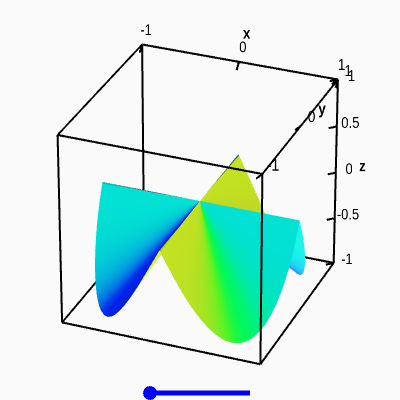
\includegraphics[width=.5\textwidth]{2-Differentiabilite-A}
  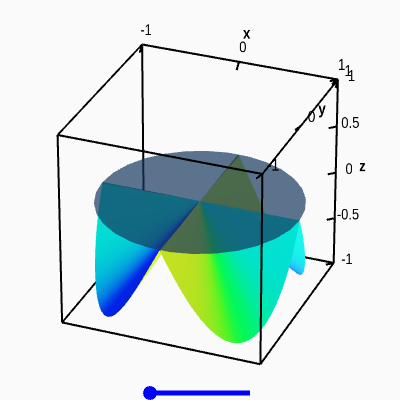
\includegraphics[width=.5\textwidth]{2-Differentiabilite-B}
  $$
  source: \url{https://mathinsight.org/differentiability_multivariable_subtleties}
  }
  \item Dans le cas de la fonction
  $$
  \begin{array}{rrcl}
    f : & \Rbb^n & \mapsto & \Rbb \\
    & x & \rightarrow & x^\top B x
  \end{array}
  $$
  on a donc montré que $J_x f = x^\top (B + B^\top)$. Dans le cas ou $B$ est symétrique, on obtient $J_x f = 2 x^\top B$ où l'on retrouve la forme de la dérivée de $bx^2$, à savoir $2 bx$.

\end{enumerate}

%-------------------------------------------------------------------------------
\exemple{[Passage en coordonnées polaires]
  Soit l'application
  $$
  \begin{array}{rrcl}
    f : & \Rbb^+ \times [0, 2\pi] & \mapsto & \Rbb^2 \\
    & (\rho, \theta) & \rightarrow & (x = \rho \cos \theta, y = \rho \sin \theta).
  \end{array}
  $$
  Sa matrice jacobienne est
  $$
  J_{(\rho, \theta)}f = \left[ \begin{array}{rclcrcl}
      \frac{\partial}{\partial \rho} \rho \cos \theta & = & \cos \theta  & &
      \frac{\partial}{\partial \theta} \rho \cos \theta & = & -\rho \sin \theta  \\
      \frac{\partial}{\partial \rho} \rho \sin \theta & = & \sin \theta  & & 
      \frac{\partial}{\partial \theta} \rho \sin \theta & = & \rho \cos \theta  
    \end{array} \right].
  $$
  On peut remarquer que
  $$
  |J_{(\rho, \theta)}f| 
  = \left| \begin{array}{cc}
      \cos \theta  & -\rho \sin \theta  \\
      \sin \theta  & \rho \cos \theta  
    \end{array} \right|
  = \rho \cos^2\theta + \rho \sin^2 \theta = \rho.
  $$
}


%-------------------------------------------------------------------------------
\remark
On peut déterminer le plan tangent à une surface $S$ de $\Rbb^3$ d'équation
$$
z = f(x, y).
$$
au point $(x_0, y_0)$, en posant $z_0 = f(x_0, y_0)$ et $h = (x-x_0, y-y0)$, soit 
$$
f(x, y) - f(x_0, x0) = \left(J_{(x_0, y_0)} f\right) \; h + o(\|h\|).
$$
Le plan tangent a ainsi pour équation
$$
z = z_0 + \frac{\partial f}{\partial x}(x_0, y_0) \times (x-x_0) + \frac{\partial f}{\partial y}(x_0, y_0) \times (y-y_0).
$$

\exemple{
Pour
$$
f(x, y) = \exp\left(-\frac{x^2 + y^2}{2}\right),
$$
on a 
$$
\frac{\partial f}{\partial x}(x_0, y_0) = - x_0 f(x_0, y_0), 
\qquad
\frac{\partial f}{\partial y}(x_0, y_0) = - y_0 f(x_0, y_0)
$$
et le plan tangent a pour équation
$$
z 
= f(x_0, y_0)(1 - x_0 (x-x_0) - y_0 (y-y_0))
= f(x_0, y_0)(1 + x_0^2 + y_0^2 - x_0 x - y_0 y)
$$
Ce plan est bien horizontal pour $(x_0, y_0) = (0, 0)$.
}

%-------------------------------------------------------------------------------
%-------------------------------------------------------------------------------
\subsection{Composition} 
%-------------------------------------------------------------------------------

On cherche maintenant à généraliser la formule connue pour deux applications $f$ et $g$ de $\Rbb$ dans $\Rbb$:
$$
(f \circ g)'(x) = g'(x) (f' \circ g)(x)
$$

\begin{proposition} \label{prop:compositionDéfferentielles}
  Si $g : \Rbb^n \mapsto \Rbb^k$ est différentiable en $x$ et $f : \Rbb^k \mapsto \Rbb^\ell$ est différentiable en $g(x)$, alors
  \begin{itemize}
   \item $f \circ g: \Rbb^n \mapsto \Rbb^\ell$ est différentiable en $x$ et
   \item sa différentielle vaut
   $$
   D_x(f \circ g) = D_{g(x)}f \circ D_xg
   $$
   et donc
   $$
   J_x(f \circ g) = J_{g(x)}f \cdot J_xg.
   $$
  \end{itemize}
\end{proposition}

Cette proposition n'est pas démontrée ici. \eproof

% \progres{
%   Début Cours 6. Rappels :
%   \begin{enumerate}[\itemdot]
%     \item Définition de l'application linéaire tangente $D_x f(h)$ telle que 
%     $$f(x+h) - f(x) - D_x f(h) = o(\|h\|).$$
%     \item Si $f$ différentiable en $x$, la matrice jacobienne $J_xf$ vérifie $D_xf(h) = J_xf \cdot h$
%     \item Exemple $f(x) = x^\top B x : J_x f = x^\top (B + B^\top) $
%     \item Exemple : calcul de $J_x f$ pour le passage en coordonnées polaires (\textcolor{red}{démontrer la différentiabilité de $f$ : cf classeur})
%     \item Composition : 
%     $$
%     D_x(f \circ g) = D_{g(x)}f \circ D_x g
%     \qquad \Rightarrow \qquad
%     J_x(f \circ g) = J_{g(x)}f \cdot D_x g.
%     $$
%     (\textcolor{red}{donner l'exempel de simple juste après})
%     \item Exercice : calculer le pente de la tangente à la courbe $(x = \rho \cos \theta, y = \rho \sin \theta)$ pour $\rho = \rho(\theta)$
%   \end{enumerate}
% }

%-------------------------------------------------------------------------------
\exemple{
Soient $f : \Rbb^k \mapsto \Rbb$ et $g : \Rbb \mapsto \Rbb^k$ telle que $g$ est différentiable en $x^*$ et $f$ en $g(x^*)$, on a
$$
J_{y^*}f = \left[\left.\frac{\partial f}{\partial y_1}\right|_{y^*} 
  \cdots 
  \left.\frac{\partial f}{\partial y_k}\right|_{y^*}  \right] 
\qquad \text{et} \qquad 
J_{x^*}g = \left[\begin{array}{c}
              \displaystyle{\left.\frac{\partial g_1}{\partial x}\right|_{x^*}}  \\
              \vdots \\
              \displaystyle{\left.\frac{\partial g_k}{\partial x}\right|_{x^*}} 
             \end{array}\right]
        = \left[\begin{array}{c} g'_1(x^*) \\ \vdots \\ g'_k(x^*) \end{array}\right]
$$
donc
$$
J_{x^*}(f \circ g) 
  = J_{g(x^*)} f \cdot J_{x^*}g
  = \left[\left.\frac{\partial f}{\partial y_1}\right|_{g(x^*)} 
    \cdots 
    \left.\frac{\partial f}{\partial y_k}\right|_{y^*}  \right] 
    \left[\begin{array}{c} g'_1(x^*) \\ \vdots \\ g'_k(x^*) \end{array}\right] 
  = \sum_{i=1}^k \left.\frac{\partial f}{\partial y_i}\right|_{g(x^*)} g'_i(x^*).
$$
}

%-------------------------------------------------------------------------------
\paragraph*{Transformation en coordonnées polaires.} 

\begin{proposition} \label{prop:differentiabiliteCoordonneesPolaires}
  La transformation en coordonnée polaire est partout différentiable sur $\Rbb^{*+} \times \Rbb^+$.
\end{proposition}

\parSR{Démonstration de la proposition \ref{prop:differentiabiliteCoordonneesPolaires}.}
Pour $u = [\rho \; \theta]^\top$ et $h = [r \; t ]^\top$, on a
$$
f(u+h) = \left[\begin{array}{c} 
    (\rho+r) \cos(\theta +t) \\ (\rho+r) \sin(\theta +t) 
    \end{array} \right]
$$
or, la fonction cosinus est partout dérivable et on a pour tout $\theta$
$$
\cos(\theta +t) = \cos \theta - t \sin \theta + o(|t|)
$$
donc
\begin{align*}
  (\rho+r) \cos(\theta +t) 
  & =  (\rho+r) (\cos \theta - t \sin \theta + o(|t|)) \\
  & = \underset{f(u)}{\underbrace{\rho \cos \theta}} 
  - \underset{\text{linéaire en $h$}}{\underbrace{\rho t \sin \theta + r \cos \theta}} 
  - \underset{= o(\|h\|) ?}{\underbrace{rt \sin \theta + (\rho + r) o(|t|)}}.
\end{align*}
En prenant $\|h\| = \|h\|_\infty = \max(|r|, |t|)$, on a clairement $|t| \leq \|h\|$, donc $o(|t|) = o(\|h\|)$. De plus
$$
\left|\frac{rt}{\|h\|}\right| 
\leq \frac{\|h\|^2}{\|h\|}
\qquad \Rightarrow \qquad 
rt = o(\|h\|).
$$
Le calcul pour $(\rho+r) \sin(\theta +t)$ est analogue.
\eproof


\exemple{
  Soit une courbe exprimée en coordonnées polaires $\rho = \rho(\theta)$. 
  \begin{enumerate}
   \item On peut déterminer les dérivées des coordonnées cartésiennes $x$ et $y$ par rapport à $\theta$ en considérant les deux applications 
  $$
  \begin{array}{rrcl}
    g : & \Rbb^+ & \mapsto & \Rbb^+ \times \Rbb^+ \\
    & \theta & \rightarrow & g(\theta) = (\rho(\theta), \theta)
  \end{array}
  $$
  et
  $$
  \begin{array}{rrcl}
    f : & \Rbb^+ \times \Rbb^+ & \mapsto & \Rbb^2 \\
    & (\rho, \theta) & \rightarrow & f(\rho, \theta) = (x = \rho \cos \theta, y = \rho \sin \theta).
  \end{array}
  $$
  On a
  $$
  J_{(\rho, \theta)}f = \left[ \begin{array}{ccc}
      \cos \theta  & & -\rho \sin \theta  \\
      \sin \theta  & & \rho \cos \theta  
    \end{array} \right]
  \text{ (déjà vu)}
  \qquad \text{et} \qquad 
  J_\theta g = \left[\begin{array}{c} \rho'(\theta) \\ 1 \end{array} \right].
  $$
  On a donc
  $$
  J_{\theta}(f \circ g) 
  = J_{(\rho(\theta), \theta)}f \cdot J_\theta g
  = \left[ \begin{array}{ccc}
      \cos \theta  & & -\rho \sin \theta  \\
      \sin \theta  & & \rho \cos \theta  
    \end{array} \right]
    \cdot
    \left[\begin{array}{c} \rho'(\theta) \\ 1 \end{array} \right]
  = \left[ \begin{array}{c}
      \rho'(\theta) \cos \theta  - \rho(\theta) \sin \theta  \\
      \rho'(\theta) \sin \theta  + \rho(\theta) \cos \theta  
    \end{array} \right]
  $$
  c'est-à-dire
  $$
  x'(\theta) = \frac{\partial x}{\partial \theta} = \rho'(\theta) \cos \theta  - \rho(\theta) \sin \theta, \qquad 
  y'(\theta) = \frac{\partial y}{\partial \theta} = \rho'(\theta) \sin \theta  + \rho(\theta) \cos \theta.
  $$
  \item La pente de la tangente à la courbe paramétrée $(x(\theta), y(\theta))$ s'obtient alors comme le rapport des dérivées partielles soit
  $$
  \frac{y'(\theta)}{x'(\theta)} 
  = \frac{\rho'(\theta) \sin \theta  + \rho(\theta) \cos \theta}{\rho'(\theta) \cos \theta  - \rho(\theta) \sin \theta}. 
  $$
  \end{enumerate}
}

%-------------------------------------------------------------------------------
\exemple{[Cas de la spirale.]
  La spirale ``linéaire'' est définie par l'équation
  $$
  \rho(\theta) = \rho_0 \theta
  \qquad \Rightarrow \qquad
  \rho'(\theta) = \rho_0,
  $$
  pour laquelle on obtient
  $$
  x'(\theta) = \rho_0 \cos \theta - \rho_0 \theta \sin \theta, \qquad 
  y'(\theta) = \rho_0 \sin \theta + \rho_0 \theta \cos \theta
  $$
  soit une pente de 
  $$
  \frac{y'(\theta)}{x'(\theta)} = \frac{\sin \theta + \theta \cos \theta}{\cos \theta - \theta \sin \theta}.
  $$
  Pour la spirale logarithmique
  $$
  \rho(\theta) = a b^\theta
  \qquad \Rightarrow \qquad
  \rho'(\theta) = a b^\theta \log b,
  $$
  on obtient
  $$
  x'(\theta) = a b^\theta \log b \cos \theta - a b^\theta \sin \theta, \qquad 
  y'(\theta) = a b^\theta \log b \sin \theta + a b^\theta \cos \theta.
  $$
  soit une pente de 
  $$
  \frac{y'(\theta)}{x'(\theta)} = \frac{\log b \sin \theta + \cos \theta}{\log b \cos \theta - \sin \theta}.
  $$
  % Pour 
  % $$
  % \rho(\theta) = \rho_0 \log(\theta)
  % \qquad \Rightarrow \qquad
  % \rho'(\theta) = \rho_0 / \theta,
  % $$
  % on obtient
  % $$
  % x'(\theta) = \frac{\rho_0 \cos \theta}{\theta} - \rho_0 \log(\theta) \sin \theta, \qquad 
  % y'(\theta) = \frac{\rho_0 \sin \theta}{\theta} + \rho_0 \log(\theta) \cos \theta.
  % $$
}

%-------------------------------------------------------------------------------
\subsection{Fonction implicite}
%-------------------------------------------------------------------------------

\begin{theorem}[Fonction implicite] \label{thm:fonctionImplicite}
  Soient $f : \Rbb^2 \mapsto \Rbb$ continuement différentiable, $\Ccal$ la courbe de niveau de $f$ associées à $c$:
  $$
  \Ccal = \{x, y: f(x, y) = c\},
  $$
  et $(x_0, y_0) \in \Rbb^2$ tels que 
  $$
  \left.\frac{\partial f}{\partial y}\right|_{x_0, y_0} \neq 0,
  $$
  il existe un voisinage $U \times V$ de $(x_0, y_0)$ et une application $\phi : \Rbb \mapsto \Rbb$ différentiable tels que, pour tout $(x, y) \in U \times V$
  $$
  (x, y) \in \Ccal \quad \Leftrightarrow \quad y = \phi(x).
  $$
  De plus
  $$
  \phi'(x) = \frac{\partial f(x, \phi(x)) / \partial x}{\partial f(x, \phi(x)) / \partial y}.
  $$
\end{theorem}

\parSR{Démonstration partielle du théorème \ref{thm:fonctionImplicite}.}
On ne démontre pas ici l'existence de $\phi$. Par contre, la détermination de sa dérivée résulte d'un calcul simple. Pour cela, on définit
$$
\begin{array}{rrcl}
  g : & \Rbb & \mapsto & \Rbb^2 \\
  & x & \rightarrow & [x \; \phi(x)]^\top.
\end{array}
$$
On a donc $f \circ g (x) = f(x, \phi(x)$ et donc
$$
(f \circ g)'(x) = \frac{\partial}{\partial x} f(x, \phi(x)) + \phi'(x) \frac{\partial}{\partial y} f(x, \phi(x)).
$$
De plus, pour $x \in U$, on a $f(x, \phi(x) = c$, donc $(f \circ g)'(x) = 0$, soit
$$
\phi'(x) = \frac{\partial f(x, \phi(x)) / \partial x}{\partial f(x, \phi(x)) / \partial y}.
$$
\eproof

